% Header: Here are all packages used and some additional definitions
%%%%%%%%%%%%%%%%%%%%%%%%%%%%%%%%%%%%%%%%%%%%%%%%%%%%%%%%%%%%%%%%%%%

\documentclass[11pt,a4paper]{article}
\usepackage[margin=2.5cm]{geometry}
\usepackage[onehalfspacing]{setspace}
\usepackage{graphicx} % zum Einbinden von Graphiken
\usepackage[breaklinks=true,colorlinks=true,linkcolor=blue,urlcolor=blue,citecolor=blue]{hyperref} % f. Referenzen
\usepackage{amsmath,amsthm,amssymb} % Mathematik Umgebung 
\usepackage{icomma} % Intelligentes Komma, das den richtigen Abstand zwischen Dezimalzahlen als auch in Formeln wählt.
\usepackage[ngerman]{babel} % Deutsche Bezeichnungen bei Inhaltsangabe etc
\usepackage[T1]{fontenc}    % andere Schriftsatzkodierung für richtige Silbentrennung bei Umlauten
\usepackage[locale = DE,space-before-unit=true,per-mode = symbol]{siunitx} % Bessere Einheiten
\usepackage{placeins} % Definiert den Befehl “\FloatBarrier”, der die Ausgabe der davor eingebundenen Bilder erzwingt, befor der Text weiter geht. (Mit vorsicht zu verwenden)
\usepackage[natbib,abbreviate=true,doi=false,style=numeric-comp,giveninits=true,sorting=none]{biblatex} % Modernes Paket zur Erzeugung von Bibliografien (benötigt biber!)
\usepackage[european, straightvoltages]{circuitikz} % Erstellung von elektrischen Schaltungen
\usepackage{pgfplots} % Erstellung von Graphen
\usepackage{float}% Ermöglicht [H] bei \figures
\pgfplotsset{compat=1.18} % Empfohlen, um die neueste Engine zu nutzen

\addbibresource{MyBibliography.bib} % Ort der .bib Datei, die die Datenbank für Literatur/Referenzen enthält.

\graphicspath{{Bilder/}}

\DeclareSIUnit{\dBm}{dBm}
\DeclareSIUnit[per-mode=reciprocal]\WN{\per\centi\meter}

%%%%%%%%%%%%%%%%%%%%%%%%%%%%%%%%%%%%%%%%%%%%%%%%%%%%%%%%%%%%%%%%%%%
\begin{document}
%
\title{
\includegraphics[width=5cm]{logo.jpg} \\ Schaltungstechnik: Ein Experimenteller Überblick}
\author{Kevin Gonci (62400675), Paul Maurer (62400670)\\Sommersemester 2026}
\date{\today}
\maketitle
\vfill
\renewcommand\abstractname{Kurzfassung}
\section*{\abstractname}
\textit{In diesem Praktikum wurden in mehreren Laborterminen verschiedene Transistorschaltungen aufgebaut, Messungen durchgeführt und die Ergebnisse diskutiert.}
\thispagestyle{empty}
%
%
\tableofcontents
\thispagestyle{empty}
\cleardoublepage
\pagenumbering{arabic} 
\newpage
%
%
\newpage

\section{Laborversuch}
% Paul
\section*{Kurzzusammenfassung}
In diesem Laborversuch wurde zunächst eine Einführung in das ordnungsgemäße Messen im Labor gegeben. Anschließend wurden die Eigenschaften des verwendeten Transistors anhand von Kennlinien beschrieben. Abschließend wurde eine Emitterverstärkerschaltung untersucht.

\section*{Durchführung}
\subsection*{1}
Zu Beginn wird eine Reihenschaltung aus zwei \SI{3,3}{\mega\ohm} Widerständen aufgebaut (siehe Abbildung \ref{Reihenschaltung}). Die exakten Widerstandswerte werden vorab mit einem Multimeter gemessen. Nach dem Anschluss einer \SI{12}{\volt} Spannungsversorgung wird der Spannungsabfall $U_{R_2}$ mithilfe eines Oszilloskops ermittelt.
\begin{figure}[H]
    \centering
    \begin{circuitikz}[european]
        \draw (0,0)
        to[V, l=$\SI{12}{\volt}$, a = $U_1$ ] (0,3)             % Spannungsquelle links
        to[R, l=$\SI{3.23}{\mega\ohm}$, a = $R_1$] (3,3)             % Erster Widerstand oben
        to[R, l=$\SI{3.20}{\mega\ohm}$, a = $R_2$] (6,3)             % Zweiter Widerstand oben (in Reihe)
        to[short] (6,0)                  % Leitung nach unten
        -- (0,0);                        % Leitung zurück zum Start
    \end{circuitikz}
    \caption{Ideale Reihenschaltung}
    \label{Reihenschaltung}
\end{figure}
Dabei wurde ein Wert von \SI{2,23}{\volt} gemessen, obwohl theoretisch ein Spannungsabfall von \SI{6}{\volt} zu erwarten gewesen wäre.

\section*{2}
Anschließend wurde die erste Transistorschaltung realisiert. Das Ziel hierbei war die experimentelle Aufnahme der Übertragungskennlinien ($U_{BE}$, $I_C$) und ($I_B$, $I_C$) des Transistors 2N4401. Als Vorwiderstand wurde ein \SI{22}{\kilo\ohm} Widerstand gewählt und die Spannung $U_{CE}$ auf \SI{5}{\volt} eingestellt. Der Kollektorstrom $I_C$ sollte dabei auf \SI{60}{\milli\ampere} limitiert werden.
Die Spannungen wurden mit dem Oszilloskop aufgezeichnet, während die Ströme über das Multimeter gemessen wurden.

\section*{3}
Im letzten Teil des ersten Laborversuchs wurde eine Emitterverstärkerschaltung mit Stromgegenkopplung sowie Emitter- und Koppelkondensator simuliert (siehe Abbildung \ref{fig:5}). Nach der Simulation wurde die Schaltung real im Labor aufgebaut, um die reale Spannungsverstärkung zu ermitteln.
\begin{figure}[H]
    \centering
    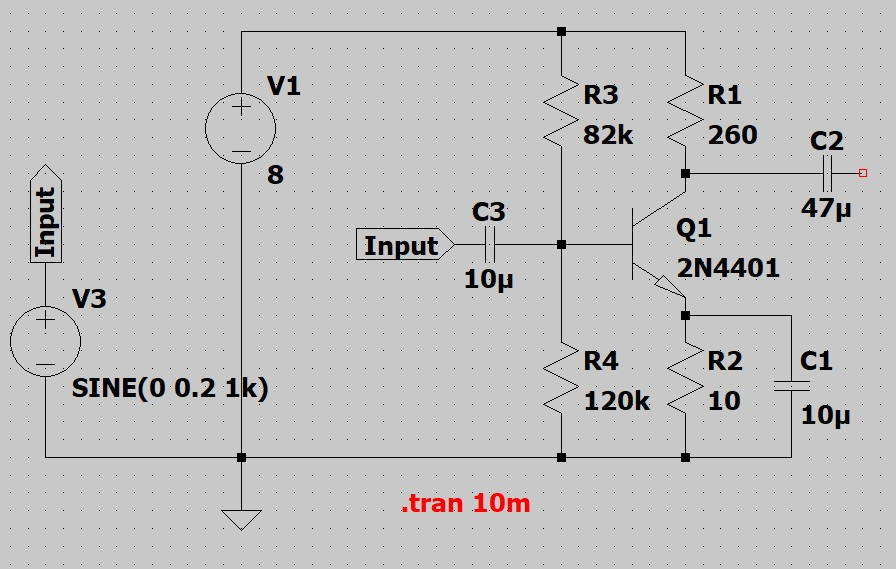
\includegraphics[width=0.4\textwidth]{Fotos 1.Labor/Emitterverstärkerschaltung.jpg}
    \caption{Schaltungsaufbau der Emitterverstärkerschaltung}
    \label{fig:5}
\end{figure}

Die Versorgungsspannung der Schaltung beträgt \qty{12}{\volt}. Als Eingangssignal diente ein Sinussignal mit einer Amplitude von \SI{20}{\milli\volt} und einer Frequenz von \SI{1}{\kilo\hertz}. Der Arbeitspunkt des Ausgangssignals sollte bei \qty{6}{\volt} liegen.
Das Eingangssignal wurde im Labor mittels eines Funktionsgenerators erzeugt, und der gewünschte Arbeitspunkt wurde über ein Potentiometer einjustiert. Das resultierende Ausgangssignal wurde abschließend mit dem Oszilloskop gemessen.

\section*{Diskussion}
\subsection*{1}
Die erhebliche Abweichung bei der Messung des Spannungsabfalls lässt sich durch den endlichen Innenwiderstand des Oszilloskop-Tastkopfes erklären, welcher im Bereich von \SI{1}{\mega\ohm} liegt. Dadurch ergibt sich für die reale Messung eine Schaltung, die aus der Reihenschaltung des Widerstands $R_1$ und einer Parallelschaltung aus $R_2$ und dem Innenwiderstand des Oszilloskops besteht (siehe Abbildung \ref{Reihenschaltung2}).
\begin{figure}[H]
    \centering
    \begin{circuitikz}[european]
        \draw
        % Spannungsquelle links
        (0,0) to[V, l=$\SI{12}{\volt}$, a= $U_1$] (0,4)
        
        % Erster Widerstand in Reihe
        to[R, l=$\SI{3.23}{\mega\ohm}$, a = $R_1$] (3,4)
        
        % Abzweigpunkt für die Parallelschaltung
        to[short, -*] (4,4) 
        
        % Oberer Zweig der Parallelschaltung
        -- (4,5) to[R, l=$\SI{3.20}{\mega\ohm}$, a = $R_2$] (7,5) -- (7,4)
        
        % Unterer Zweig der Parallelschaltung
        (4,4) -- (4,3) to[R, l=$\SI{957947}{\ohm}$, a = $R_3$] (7,3) -- (7,4)
        
        % Rückleitung zum Minuspol
        node[circ] {} -- (8,4) % Verbindungspunkt Ende
        to[short] (8,0) 
        -- (0,0);
    \end{circuitikz}
    \caption{Reale Schaltungsstruktur unter Berücksichtigung des Messgerätes}
    \label{Reihenschaltung2}
\end{figure}
Der exakte Wert dieses Innenwiderstands ($R_3$) lässt sich durch Umstellen der Spannungsteilerregel nach den Gleichungen \ref{eq:1} bis \ref{eq:3} rechnerisch ermitteln:
\begin{equation}
    U_{R_2,R_3}= \frac{R_2 \parallel R_3}{R_1 + R_2 \parallel R_3} \cdot U_1 = \frac{R_2 \cdot R_3}{R_1 \cdot R_2 + R_1 \cdot R_3 + R_2 \cdot R_3} \cdot U_1
    \label{eq:1}
\end{equation}
\begin{equation}
    \frac{U_{R_2,R_3}}{U_1} \cdot (R_1 \cdot R_2 + R_1 \cdot R_3 + R_2 \cdot R_3) - R_2 \cdot R_3 = 0
    \label{eq:2}
\end{equation}
\begin{equation}
    R_3 = \frac{\frac{U_{R_2,R_3}}{U_1} \cdot R_1 \cdot R_2}{R_2 - \frac{U_{R_2,R_3}}{U_1} \cdot (R_1 + R_2)} = \SI{957947,891}{\ohm}
    \label{eq:3}
\end{equation}

\subsection*{2}
Die messtechnisch erfassten Werte für die Übertragungs- und die Stromverstärkungskennlinie sind in Abbildung \ref{fig:1} grafisch dargestellt.
\begin{figure}[H]
\centering
        \begin{tikzpicture}
        \begin{axis}[
            width = 0.46\textwidth,
            xlabel={$U_{BE}$\; [V]},
            ylabel={$I_C$ \; [mA]},
            grid=both,          % Zeigt Haupt- und Hilfslinien an
            minor tick num=1    % Fügt kleine Zwischenschritte im Gitter hinzu
        ]
        \addplot[
            color=red,          % Farbe der Linie
            thick,              % Macht die Linie etwas dicker
            mark=*,             % Markiert die Datenpunkte mit einem Punkt
        ]
        coordinates {
            (0.488, 0)
            (0.552, 0.1)
            (0.568, 0.2)
            (0.592, 0.3)
            (0.6  , 0.5)
            (0.608, 0.6)
            (0.616, 0.8)
            (0.624, 1.1)
            (0.632, 1.5)
            (0.64 , 2.2)
            (0.656, 3.8)
            (0.664, 5.6)
            (0.672, 16.7)
            (0.68 , 21.3)
        };
        \addlegendentry{Übertragungskennlinie}
        \end{axis}
        \end{tikzpicture} 
        \begin{tikzpicture}
        \begin{axis}[
            width = 0.46\textwidth,
            xlabel={$I_B$\; [mA]},
            ylabel={$I_C$ \; [mA]},
            grid=both,          % Zeigt Haupt- und Hilfslinien an
            minor tick num=1    % Fügt kleine Zwischenschritte im Gitter hinzu
        ]
        \addplot[
            color=green,          % Farbe der Linie
            thick,              % Macht die Linie etwas dicker
            mark=*,             % Markiert die Datenpunkte mit einem Punkt
        ]
        coordinates {
            (0.01 ,  0.8)
            (0.02 ,  3.1)
            (0.03 ,  6.6)
            (0.04 ,  7.6)
            (0.05 ,  9.4)
            (0.06 , 11.1)
            (0.07 , 13.9)
            (0.08 , 15.8)
            (0.09 , 17.6)
            (0.1  , 18.6)
            (0.11 , 21.5)
            (0.12 , 24.5)
            (0.13 , 25.7)
            (0.14 , 27.6)
            (0.15 , 29.6)
            (0.16 , 33.6)
            (0.17 , 35.7)
            (0.18 , 37.1)
            (0.19 , 39.1)
            (0.2  , 41.2)
            (0.21 , 45.3)
            (0.22 , 46.5)
            (0.23 , 48.6)
            (0.24 , 50.8)
        };
        \addlegendentry{Stromverstärkungskennlinie}
        \end{axis}
        \end{tikzpicture} 
    \caption{Messtechnisch ermittelte Übertragungskennlinien}
    \label{fig:1}
\end{figure}

Anhand der Übertragungskennlinie in Abbildung \ref{fig:1} wird das charakteristische exponentielle Verhalten des Kollektorstroms im Verhältnis zur Basis-Emitter-Spannung deutlich. Die Stromverstärkungskennlinie (siehe Abbildung \ref{fig:1}) weist hingegen einen näherungsweise linearen Verlauf auf. Ein steigender Basisstrom resultiert folglich in einem proportional ansteigenden Kollektorstrom.

Zum Vergleich wurde das Systemverhalten in LTspice simuliert (siehe Abbildung \ref{fig:2}). Die Simulationswerte zeigen eine gute Übereinstimmung mit den realen Messwerten. Geringfügige Abweichungen lassen sich auf Bauteiltoleranzen sowie thermische Einflüsse im Laborbetrieb zurückführen.
\begin{figure}[H]
    \centering
    \begin{tikzpicture}
        \begin{axis}[
            width=0.46\textwidth,
            xlabel={$U_{BE}$ [V]},
            ylabel={$I_C$ [mA]},
            grid=both,
            minor tick num=1,
            table/col sep=tab, 
            scaled y ticks=true,
        ]
        \addplot[
            color=red,          
            thick,              
            ] table [x index=1, y expr=\thisrowno{2}*1000] {Simulationen 1.Labor/sim1.txt};
            
        \addlegendentry{Übertragungskennlinie}
        \end{axis}
    \end{tikzpicture}
    \begin{tikzpicture}
        \begin{axis}[
            width=0.46\textwidth,
            xlabel={$I_B$ [mA]},
            ylabel={$I_C$ [mA]},
            grid=both,
            minor tick num=1,
            table/col sep=tab, 
            scaled y ticks=true,
        ]
        \addplot[
            color=green,          
            thick,              
            ] table [x expr=\thisrowno{1}*1000, y expr=\thisrowno{2}*1000] {Simulationen 1.Labor/sim2.txt};
            
        \addlegendentry{Stromverstärkungskennlinie}
        \end{axis}
    \end{tikzpicture}
    \caption{Simulierte Übertragungskennlinien (LTspice)}
    \label{fig:2}
\end{figure}

Des Weiteren wurden auf Basis der Simulationsdaten die Eingangskennlinie sowie das Ausgangskennlinienfeld generiert (siehe Abbildung \ref{fig:3}).
Auch die Eingangskennlinie verdeutlicht das exponentielle Diodenverhalten der Basis-Emitter-Strecke. Im Ausgangskennlinienfeld lässt sich in Abhängigkeit von der angelegten Basis-Emitter-Spannung der Übergang des Transistors in den Sättigungsbereich exakt ablesen.
\begin{figure}[H]
    \centering
    \begin{tikzpicture}
        \begin{axis}[
            width = 0.46\textwidth,
            xlabel={$U_{BE}$ [V]},
            ylabel={$I_B$ [mA]},
            grid=both,
            minor tick num=1,
            table/col sep=tab, 
            scaled y ticks=true,
        ]
        \addplot[
            color=blue,          
            thick,              
            ] table [x index=1, y expr=\thisrowno{2}*1000] {Simulationen 1.Labor/Eingangskennlinie.txt};
        \addlegendentry{Eingangskennlinie}
        \end{axis}
    \end{tikzpicture}
    \begin{tikzpicture}
        \begin{axis}[
            width = 0.5\textwidth,
            xlabel={$U_{CE}$ [V]},
            ylabel={$I_C$ [mA]},
            grid=both,
            minor tick num=1,
            table/col sep=tab, 
            scaled y ticks=true,
        ]
        \addplot[
            color=green,          
            thick,              
            ] table [x index=1, y expr=\thisrowno{2}*1000] {Simulationen 1.Labor/Ausgangskennlinie1.txt};
            \addlegendentry{$U_{BE}$=\SI{660}{\milli\volt}}
        \addplot[
            color=violet,          
            thick,              
            ] table [x index=1, y expr=\thisrowno{2}*1000] {Simulationen 1.Labor/Ausgangskennlinie3.txt};
            \addlegendentry{$U_{BE}$=\SI{715}{\milli\volt}}
        \addplot[
            color=red,         
            thick,              
            ] table [x index=1, y expr=\thisrowno{2}*1000] {Simulationen 1.Labor/Ausgangskennlinie5.txt};
            \addlegendentry{$U_{BE}$=\SI{770}{\milli\volt}}
        \addplot[
            color=cyan,          
            thick,              
            ] table [x index=1, y expr=\thisrowno{2}*1000] {Simulationen 1.Labor/Ausgangskennlinie7.txt};
            \addlegendentry{$U_{BE}$=\SI{825}{\milli\volt}}
        \addplot[
            color=orange,          
            thick,              
            ] table [x index=1, y expr=\thisrowno{2}*1000] {Simulationen 1.Labor/Ausgangskennlinie9.txt};
            \addlegendentry{$U_{BE}$=\SI{880}{\milli\volt}}
        \end{axis}
    \end{tikzpicture}
    \caption{Simulierte Eingangs- und Ausgangskennlinien}
    \label{fig:3}
\end{figure}

Zusätzlich wurde aus den extrahierten Simulationsdaten ein Vierquadranten-Kennlinienfeld erstellt (siehe Abbildung \ref{fig:4}). Hierbei ist im ersten Quadranten das Ausgangskennlinienfeld (orange, violett, rot) abgebildet, welches zur besseren Übersicht auf den Bereich $U_{BE} = \SI{660}{\milli\volt}$ bis \SI{715}{\milli\volt} begrenzt wurde. Der zweite Quadrant stellt die Stromverstärkungskennlinie (grün) dar, während im dritten Quadranten die exponentielle Eingangskennlinie (blau) aufgetragen ist.
\begin{figure}[H]
    \centering
    \begin{tikzpicture}
    \begin{axis}[
        width=0.9\textwidth,
        axis lines=middle,
        xmin=-1.2, xmax=1.2,   
        ymin=-25, ymax=25, 
        grid=both,
        minor tick num=1,
        xticklabel={$\pgfmathparse{abs(\tick)}\pgfmathprintnumber{\pgfmathresult}$},
        yticklabel={$\pgfmathparse{abs(\tick)}\pgfmathprintnumber{\pgfmathresult}$},
        clip=false,
        table/col sep=tab
    ]
         \addplot[
            restrict x to domain=0:1.2,
            restrict y to domain=0:25,
            color=orange,          
            thick,              
            ] table [x index=1, y expr=\thisrowno{2}*1000] {Simulationen 1.Labor/Ausgangskennlinie1.txt};
            \addlegendentry{$U_{BE}$=\SI{660}{\milli\volt}}
        \addplot[
            restrict x to domain=0:1.2,
            restrict y to domain=0:25,
            color=violet,          
            thick,              
            ] table [x index=1, y expr=\thisrowno{2}*1000] {Simulationen 1.Labor/Ausgangskennlinie2.txt};
            \addlegendentry{$U_{BE}$=\SI{687.5}{\milli\volt}}
        \addplot[
            restrict x to domain=0:1.2,
            restrict y to domain=0:25,
            color=red,         
            thick,              
            ] table [x index=1, y expr=\thisrowno{2}*1000] {Simulationen 1.Labor/Ausgangskennlinie3.txt};
            \addlegendentry{$U_{BE}$=\SI{715}{\milli\volt}}
         \addplot[
            restrict y to domain=0:25,
            color=green,          
            thick,              
            ] table [x expr=\thisrowno{1}*-1000, y expr=\thisrowno{2}*1000] {Simulationen 1.Labor/sim2.txt};
        \addplot[
            restrict x to domain=-1.19:0,
            color=blue,          
            thick,              
            ] table [x expr=\thisrowno{1}*-1, y expr=\thisrowno{2}*-1000] {Simulationen 1.Labor/Eingangskennlinie.txt};
        
        % Manuelle Beschriftungen der Quadranten-Achsen
        \node[anchor=south west] at (rel axis cs:1, 0.5) {$U_{CE}$ [V]};
        \node[anchor=south east] at (rel axis cs:0, 0.5) {$I_{B}$ [mA]};
        \node[anchor=south west] at (rel axis cs:0.5, 1) {$I_C$ [mA]};
        \node[anchor=north west] at (rel axis cs:0.5, 0) {$U_{BE}$ [V]};
    \end{axis}
\end{tikzpicture}
\caption{Vierquadranten-Kennlinienfeld (Simulation)}
\label{fig:4}
\end{figure}

\subsection*{3}
Die Simulationsergebnisse der Emitterschaltung zeigen ein phasenverschobenes, sinusförmiges Ausgangssignal mit deutlich vergrößerter Amplitude (siehe Abbildung \ref{fig:6}).
\begin{figure}[H]
    \centering
    \begin{tikzpicture}
        \begin{axis}[
            width=0.50\textwidth,
            xlabel={$t$ [s]},
            ylabel={$U$ [V]},
            grid=both,
            minor tick num=1,
            table/col sep=tab, 
            scaled y ticks=true,
            legend pos = outer north east,
        ]
        \addplot[
            color=red,          
            thick,              
            ] table [x index=0, y index=1] {Simulationen 1.Labor/Emitter.txt};
        \addlegendentry{Eingangsspannung}
        \addplot[
            color=blue,          
            thick,              
            ] table [x index=0, y index=2] {Simulationen 1.Labor/Emitter.txt};
        \addlegendentry{Ausgangsspannung}
        \end{axis}
    \end{tikzpicture}
    \caption{Ein- und Ausgangssignal der Emitterschaltung (Simulation)}
    \label{fig:6}
    \end{figure}
Die Spannungsverstärkung der simulierten Schaltung beläuft sich auf $A = 23,25$, wie aus Berechnung \ref{eq:4} hervorgeht:
\begin{equation}
    A = \frac{U_{A,PP}}{U_{E,PP}} = \frac{\SI{4,5}{\volt} - \SI{3,57}{\volt}}{\SI{0,02}{\volt} - (-\SI{0,02}{\volt})} = \frac{\SI{0,93}{\volt}}{\SI{0,04}{\volt}} = 23,25
    \label{eq:4}
\end{equation}
Bei der praktischen Überprüfung der Schaltung im Labor ergab sich eine reale Spannungsverstärkung von $A \approx 21,88$ (siehe Berechnung \ref{eq:5}).
\begin{equation}
    A = \frac{U_{A,PP}}{U_{E,PP}} = \frac{\SI{525}{\milli\volt}}{\SI{24}{\milli\volt}} \approx 21,875
    \label{eq:5}
\end{equation}
\newpage
% Kevin
\section{Laborversuch}
Hier kommt alles zum zweiten Laborversuch

\begin{itemize}
    \item Kurzzusammenfassung
    \item Durchführung
    \item Diskussion
\end{itemize}

\section*{Zusammenfassung}

\section*{Durchführung}
\subsection*{1}
lorem ipsum

\subsection*{2}
lorem ipsum
\newpage

\section{Laborversuch}
Hier kommt alles zum dritten Laborversuch

\section*{Kurzzusammenfassung} 
        In diesem Laborversuch wurde eine astabile Multivibratorschaltung 
        mit einem LM358 Operationsvertärker aufgebaut. 
        Diese Schaltung erzeugt ein Rechtecksignal ohne ein externes Eingangssignal.
        Anschließend wurde die Bandbreite des LM358 bei einer Verstärkung von 1
        und die Bandbreite bei einer Verstärkung von 10 gemessen. Zum Schluss wurde die 
        Input-Offset-Voltage des OPV gemessen.
\section*{Durchführung} 
        \subsection*{1}
        Zu Beginn wurde die Schaltung des astabilen Multivibrator aufgebaut. 
        Dafür wurde eine negative Spannung von \qty{5}{\volt} benötigt. Diese wurde mithilfe 
        von einer 2-Kanal-Gleichsspannungsversorgung, welche galvanisch getrennte Kanäle besitzt, 
        erzeugt. Dabei wurde der positive Anschluss des Kanal 1 
        mit dem negativen Anschluss des Kanal 2 verbunden. Der positive Anschluss des Kanal 2 war somit \qty{5}{\volt}  
        und der negative Anschluss des Kanal 1 war somit \qty{-5}{\volt}. 
        Als Ground wurde der Ausgang der negative Ausgang des Kanal 2 verwendet. 
        Anschließend wurde die Schaltung aufgebaut und mit der Gleichspannungsquelle betrieben. 
        Mit dem Oszilloskop wurde die Spannung über den Kondensator gemessen und die Spannung am Ausgang des Operationsvertärker, siehe \ref{fig:7}.
\begin{figure}

        
        \label{fig:7}
\end{figure}
        Die Schaltung besteht aus zwei Teilen der Teil des OPV der in Mitkopplung betrieben wird
        ist ein Schmitt-Trigger. Dieser ermöglicht es das die Schaltung ab einer bestimmten Spannungsschwelle schaltet.
        Diese Spannungsschwelle berechnet sich mit folgender Formel:
        \begin{equation}
               $ r_1 = $
        \end{equation}



\section*{Diskussion}

\newpage

\section{Laborversuch}
Hier kommt alles zum vierten Labor

\begin{itemize}
    \item Kurzzusammenfassung
    \item Durchführung
    \item Diskussion
\end{itemize}





\printbibliography[]
\vfill




\end{document}
